\documentclass[a4paper,11pt]{article}

% load packages
\usepackage[utf8]{inputenc}
\usepackage{amsmath}
\usepackage{amssymb}
\usepackage{array}
\usepackage{mathtools}
\usepackage{bbm}
\usepackage{float}

% define own colors and use colored text
\usepackage{xcolor}

\usepackage{tikz}
\usetikzlibrary{arrows}
\usetikzlibrary{positioning}
\usetikzlibrary{shapes}
\usetikzlibrary{fit}
\usetikzlibrary{backgrounds}

%%% standard additional commands
%epsilon
\newcommand*{\oldepsilon}{\epsilon}%
\renewcommand*{\epsilon}{\varepsilon}%

% Number Sets
\newcommand{\R}{\mathbb{R}}
\newcommand{\Z}{\mathbb{Z}}
\newcommand{\Q}{\mathbb{Q}}
\newcommand{\N}{\mathbb{N}}
\newcommand{\C}{\mathbb{C}}
\newcommand{\1}{\mathbf{1}}

% Statistics
\newcommand{\Var}{\mathbb{V}}
\newcommand{\Exp}{\mathbb{E}}

% Matrices
\newcommand{\X}{\mathbf{X}}
\newcommand{\Y}{\mathbf{Y}}

% operators
\DeclareMathOperator{\cov}{cov}
\DeclareMathOperator{\di}{d}



\begin{document}

\section{Description}
The Dunning-Kruger effect is stated in terms of skill and overconfidence to show that measurement error can cause significant bias in the relationship between performance and overestimation.
Instrumental variable methods can be used to correct for this bias.

\section{Ontology}
The constructs used are
\begin{itemize}
 \item performance as a test score
 \item performance estimation as the difference between the expected and the actual test score
 \item skill as the ability to perform well on a given test
 \item overconfidence as the difference between self-assessed and actual skill
 \item measurement error as luck on a test
\end{itemize}

\section{Relationships}

\subsection{Original DK Paper}

\begin{figure}[H]
  \vspace{1cm}
  \begin{center}
  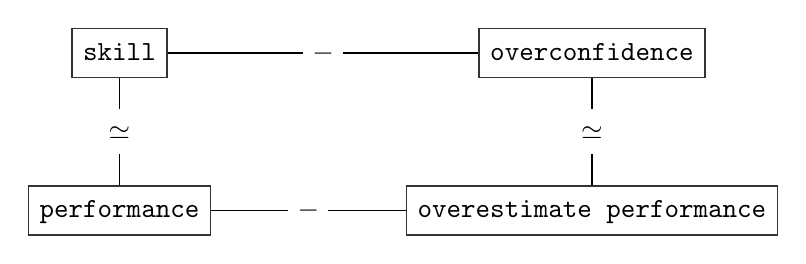
\begin{tikzpicture}
        [manifest/.style={rectangle,draw=black!80,semithick,minimum width=1cm,inner sep=4pt,text centered},
        latent/.style={circle,draw=black!80,thick,inner sep=2,text centered},
        latent_wide/.style={circle,draw=black!80,thick,inner sep=4,text centered},
        from/.style={<-,>=stealth',semithick},
        text height=1.75ex, text depth=.5ex]

\begin{scope}

% types
\node[manifest] at (0,0) (skill) {\texttt{skill}};

\node[manifest] at (6, 0) (overconfidence) {\texttt{overconfidence}};

\node[manifest] at (0, -2) (performance) {\texttt{performance}};

\node[manifest] at (6,-2) (estimate) {\texttt{overestimate performance}};


%arrows
\draw[-,>=stealth',semithick] (skill) -- node [fill=white] {$-$} (overconfidence);
\draw[-,>=stealth',semithick] (performance) -- node [fill=white] {$-$} (estimate);
\draw[-,>=stealth',semithick] (skill) -- node [fill=white] {$\simeq$} (performance);
\draw[-,>=stealth',semithick] (overconfidence) -- node [fill=white] {$\simeq$} (estimate);



\end{scope}

\end{tikzpicture}

  \end{center}
  %\caption{Subtypes of `AbstractSem`.}
  \label{fig:typetree}
\end{figure}

With $-$ signifying a negative association and $\simeq$ signifying measured by.

\begin{itemize}
 \item low skilled are more overconfident in assessing their skill than high skilled
\end{itemize}

\subsection{Formulation using measurement error}

\begin{figure}[H]
  \vspace{1cm}
  \begin{center}
  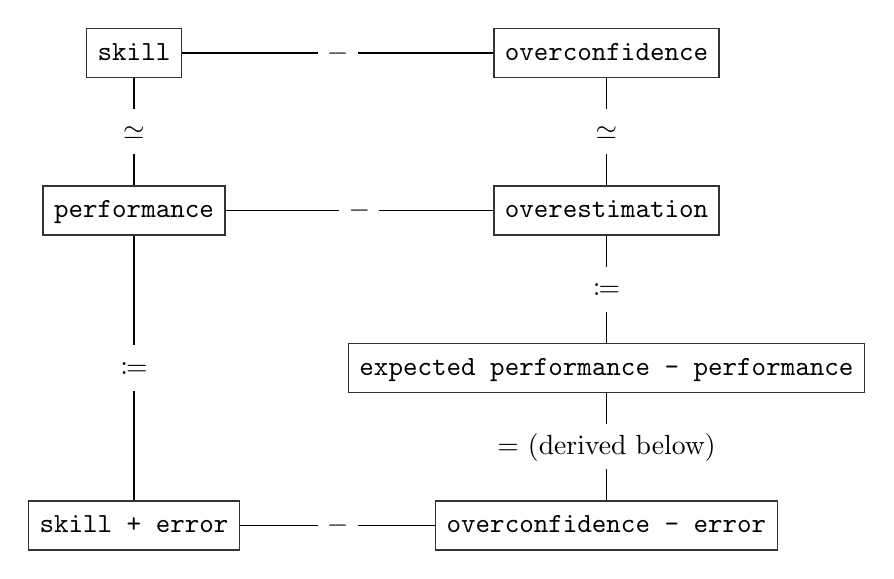
\begin{tikzpicture}
        [manifest/.style={rectangle,draw=black!80,semithick,minimum width=1cm,inner sep=4pt,text centered},
        latent/.style={circle,draw=black!80,thick,inner sep=2,text centered},
        latent_wide/.style={circle,draw=black!80,thick,inner sep=4,text centered},
        from/.style={<-,>=stealth',semithick},
        text height=1.75ex, text depth=.5ex]

\begin{scope}

% types
\node[manifest] at (0,0) (skill) {\texttt{skill}};

\node[manifest] at (6, 0) (overconfidence) {\texttt{overconfidence}};

\node[manifest] at (0, -2) (performance) {\texttt{performance}};

\node[manifest] at (6,-2) (estimate) {\texttt{overestimation}};

\node[manifest] at (0, -6) (skillerror) {\texttt{skill + error}};

\node[manifest] at (6, -4) (pminusp) {\texttt{expected performance - performance}};

\node[manifest] at (6, -6) (ocerror) {\texttt{overconfidence - error}};


%arrows
\draw[-,>=stealth',semithick] (skill) -- node [fill=white] {$-$} (overconfidence);
\draw[-,>=stealth',semithick] (performance) -- node [fill=white] {$-$} (estimate);
\draw[-,>=stealth',semithick] (skill) -- node [fill=white] {$\simeq$} (performance);
\draw[-,>=stealth',semithick] (overconfidence) -- node [fill=white] {$\simeq$} (estimate);
\draw[-,>=stealth',semithick] (skillerror) -- node [fill=white] {$-$} (ocerror);
\draw[-,>=stealth',semithick] (performance) -- node [fill=white] {$\coloneq$} (skillerror);
\draw[-,>=stealth',semithick] (estimate) -- node [fill=white] {$\coloneq$} (pminusp);
\draw[-,>=stealth',semithick] (pminusp) -- node [fill=white] {$=$ (derived below)} (ocerror);

\end{scope}

\end{tikzpicture}

  \end{center}
  \caption{A caption}
  \label{fig:typetree}
\end{figure}

\section{Mathematical Formulation}
Define random variables
\begin{itemize}
 \item $s^*$ denoting skill
 \item $\epsilon$ denoting measurement error, with $\Exp[\epsilon] = 0$, $\epsilon$ independent of all other random variables included in the model
 \item $s^*_s$ denoting self-assessed skill
\end{itemize}

\noindent Then we define performance $p$ as
\begin{equation} \label{p}
  p \coloneq s^* + \epsilon
\end{equation}
and overconfidence $oc^*$ as
\begin{equation} \label{oc}
  oc^* \coloneq s^*_s-s^*
\end{equation}
and expected performance $p_e$ as
\begin{equation} \label{ep}
  p_e \coloneq s^* + oc^*
\end{equation}
Overconfidence $oc^*$ is measured by overestimation $oe$ defined as
\begin{equation}
  oe \coloneq p_e - p
\end{equation}

\noindent From eq. \ref{oc} and \ref{ep} it follows that $p_e = s^*_s$ and further from eq. \ref{ep} and \ref{p} we see
\begin{align}
  oe &= p_e - p \\
  &= (s^* + oc^*) - (s^* + \epsilon) \\
  &= oc^* - \epsilon
\end{align}
\section{(Statistical) Models}


\subsection{Correction}
There are different ways to correct for the bias introduced by measurement error:
\begin{itemize}
 \item use different test performances to calculate skill and overconfidence, but a small test-retest correlation can bias the estimate towards zero then (Krueger and Mueller, 2002)
\end{itemize}

\section{Common Experimental Paradigm}
\begin{itemize}
 \item participants take a test
 \item participants guess their test performance either before or after the test
 \item bottom quartile performers vastly overestimate their performance, while top quartile performers access their performance more accurately
\end{itemize}

There are many replications for different populations and different tasks.

\section{Open Questions / Ambiguities}

\section{Notes}
\begin{itemize}
 \item difference in metacognitive skills drives the relationship between skill and overconfidence
\end{itemize}


\end{document}
